\documentclass{standalone}
\usepackage{tikz}
\usetikzlibrary{patterns, positioning}

\begin{document}
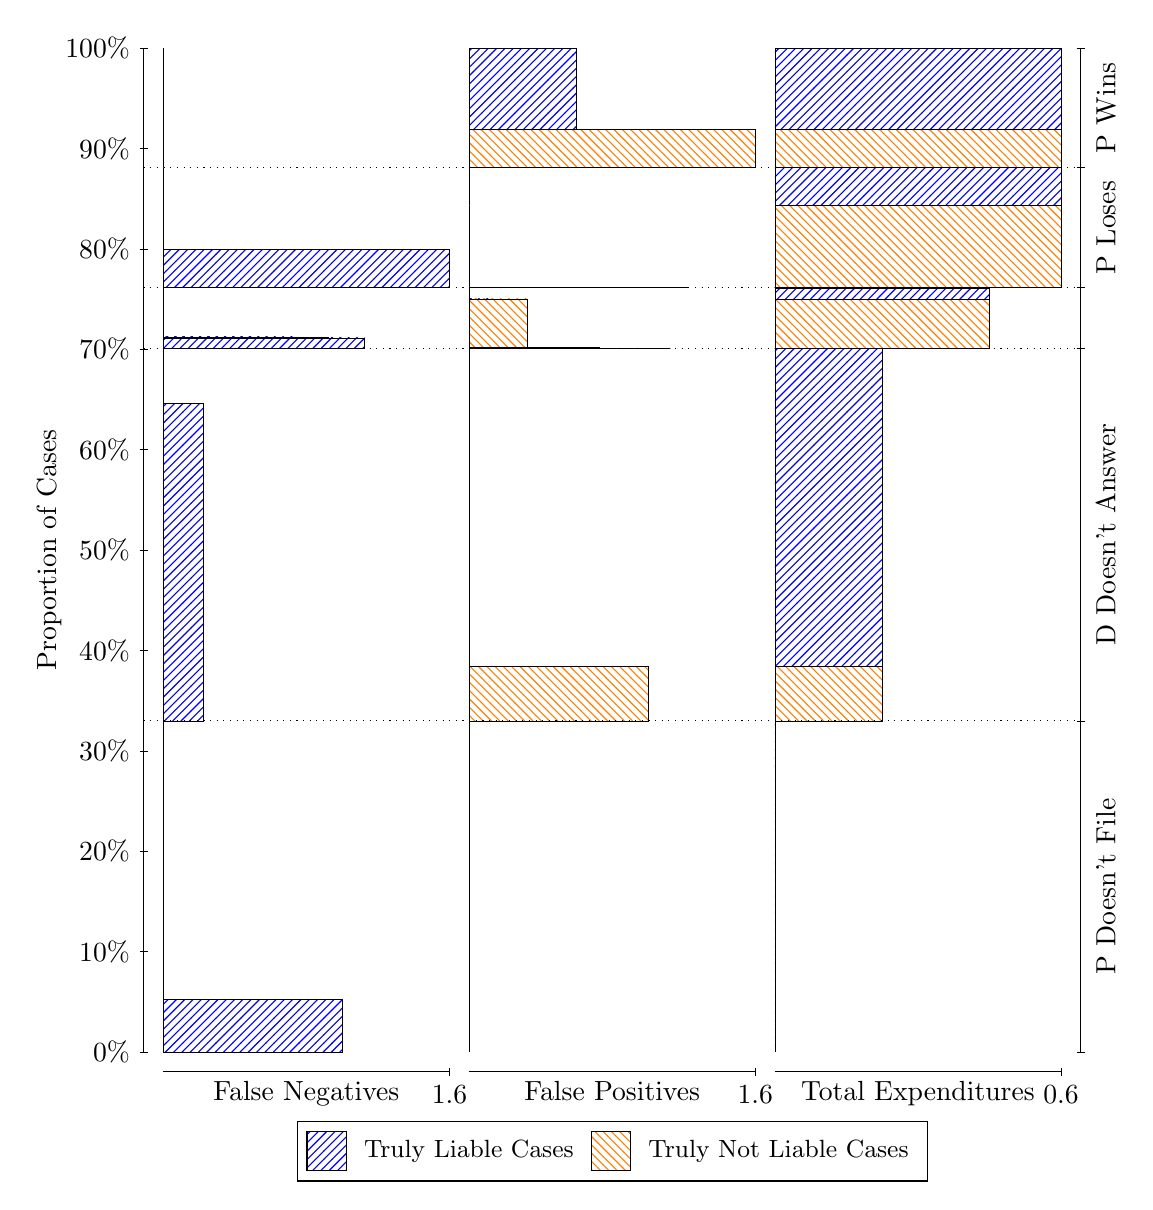
\begin{tikzpicture}
\draw[black, very thin] (1.5,1.75) -- (1.5,14.5);
\node[rotate=90, anchor=center] at (0.3, 8.125) {Proportion of Cases};
\draw[black, very thin] (1.45,1.75) -- (1.55,1.75);
\node[anchor=east] at (1.45, 1.75) {0\%};
\draw[black, very thin] (1.45,3.025) -- (1.55,3.025);
\node[anchor=east] at (1.45, 3.025) {10\%};
\draw[black, very thin] (1.45,4.3) -- (1.55,4.3);
\node[anchor=east] at (1.45, 4.3) {20\%};
\draw[black, very thin] (1.45,5.575) -- (1.55,5.575);
\node[anchor=east] at (1.45, 5.575) {30\%};
\draw[black, very thin] (1.45,6.85) -- (1.55,6.85);
\node[anchor=east] at (1.45, 6.85) {40\%};
\draw[black, very thin] (1.45,8.125) -- (1.55,8.125);
\node[anchor=east] at (1.45, 8.125) {50\%};
\draw[black, very thin] (1.45,9.4) -- (1.55,9.4);
\node[anchor=east] at (1.45, 9.4) {60\%};
\draw[black, very thin] (1.45,10.675) -- (1.55,10.675);
\node[anchor=east] at (1.45, 10.675) {70\%};
\draw[black, very thin] (1.45,11.95) -- (1.55,11.95);
\node[anchor=east] at (1.45, 11.95) {80\%};
\draw[black, very thin] (1.45,13.225) -- (1.55,13.225);
\node[anchor=east] at (1.45, 13.225) {90\%};
\draw[black, very thin] (1.45,14.5) -- (1.55,14.5);
\node[anchor=east] at (1.45, 14.5) {100\%};

\draw[black, very thin] (13.4,1.75) -- (13.4,14.5);
\draw[black, very thin] (13.35,1.75) -- (13.45,1.75);
\node[anchor=west] at (13.35, 1.75) {};
\draw[black, very thin] (13.35,5.955) -- (13.45,5.955);
\node[anchor=west] at (13.35, 5.955) {};
\draw[black, very thin] (13.35,10.684) -- (13.45,10.684);
\node[anchor=west] at (13.35, 10.684) {};
\draw[black, very thin] (13.35,11.459) -- (13.45,11.459);
\node[anchor=west] at (13.35, 11.459) {};
\draw[black, very thin] (13.35,11.459) -- (13.45,11.459);
\node[anchor=west] at (13.35, 11.459) {};
\draw[black, very thin] (13.35,12.981) -- (13.45,12.981);
\node[anchor=west] at (13.35, 12.981) {};
\draw[black, very thin] (13.35,14.5) -- (13.45,14.5);
\node[anchor=west] at (13.35, 14.5) {};

\draw[black, very thin, pattern color=blue, pattern=north east lines] (1.75,1.75) rectangle (4.0208,2.4225);
\draw[black, very thin, pattern color=orange, pattern=north west lines] (1.75,2.4225) rectangle (1.75,5.955);
\draw[black, very thin, pattern color=blue, pattern=north east lines] (1.75,5.955) rectangle (2.2609,9.9917);
\draw[black, very thin, pattern color=orange, pattern=north west lines] (1.75,9.9917) rectangle (1.75,10.684);
\draw[black, very thin, pattern color=blue, pattern=north east lines] (1.75,10.684) rectangle (4.3047,10.818);
\draw[black, very thin, pattern color=blue, pattern=north east lines] (1.75,10.818) rectangle (4.0776,10.818);
\draw[black, very thin, pattern color=blue, pattern=north east lines] (1.75,10.818) rectangle (3.8505,10.821);
\draw[black, very thin, pattern color=blue, pattern=north east lines] (1.75,10.821) rectangle (3.6234,10.821);
\draw[black, very thin, pattern color=blue, pattern=north east lines] (1.75,10.821) rectangle (3.3964,10.831);
\draw[black, very thin, pattern color=blue, pattern=north east lines] (1.75,10.831) rectangle (3.1693,10.831);
\draw[black, very thin, pattern color=blue, pattern=north east lines] (1.75,10.831) rectangle (2.9422,10.831);
\draw[black, very thin, pattern color=blue, pattern=north east lines] (1.75,10.831) rectangle (2.7151,10.831);
\draw[black, very thin, pattern color=blue, pattern=north east lines] (1.75,10.831) rectangle (2.488,10.831);
\draw[black, very thin, pattern color=orange, pattern=north west lines] (1.75,10.831) rectangle (1.75,11.459);
\draw[black, very thin, pattern color=blue, pattern=north east lines] (1.75,11.459) rectangle (2.2609,11.459);
\draw[black, very thin, pattern color=orange, pattern=north west lines] (1.75,11.459) rectangle (1.75,11.459);
\draw[black, very thin, pattern color=blue, pattern=north east lines] (1.75,11.459) rectangle (5.3833,11.94);
\draw[black, very thin, pattern color=orange, pattern=north west lines] (1.75,11.94) rectangle (1.75,12.981);
\draw[black, very thin, pattern color=orange, pattern=north west lines] (1.75,12.981) rectangle (1.75,13.462);
\draw[black, very thin, pattern color=blue, pattern=north east lines] (1.75,13.462) rectangle (1.75,14.5);
\draw[black, very thin, pattern color=orange, pattern=north west lines] (5.6333,1.75) rectangle (5.6333,5.2825);
\draw[black, very thin, pattern color=blue, pattern=north east lines] (5.6333,5.2825) rectangle (5.6333,5.955);
\draw[black, very thin, pattern color=orange, pattern=north west lines] (5.6333,5.955) rectangle (7.9042,6.6473);
\draw[black, very thin, pattern color=blue, pattern=north east lines] (5.6333,6.6473) rectangle (5.6333,10.684);
\draw[black, very thin, pattern color=orange, pattern=north west lines] (5.6333,10.684) rectangle (8.188,10.684);
\draw[black, very thin, pattern color=orange, pattern=north west lines] (5.6333,10.684) rectangle (7.9609,10.684);
\draw[black, very thin, pattern color=orange, pattern=north west lines] (5.6333,10.684) rectangle (7.7339,10.684);
\draw[black, very thin, pattern color=orange, pattern=north west lines] (5.6333,10.684) rectangle (7.5068,10.684);
\draw[black, very thin, pattern color=orange, pattern=north west lines] (5.6333,10.684) rectangle (7.2797,10.694);
\draw[black, very thin, pattern color=orange, pattern=north west lines] (5.6333,10.694) rectangle (7.0526,10.694);
\draw[black, very thin, pattern color=orange, pattern=north west lines] (5.6333,10.694) rectangle (6.8255,10.699);
\draw[black, very thin, pattern color=orange, pattern=north west lines] (5.6333,10.699) rectangle (6.5984,10.699);
\draw[black, very thin, pattern color=orange, pattern=north west lines] (5.6333,10.699) rectangle (6.3714,11.313);
\draw[black, very thin, pattern color=blue, pattern=north east lines] (5.6333,11.313) rectangle (5.9172,11.313);
\draw[black, very thin, pattern color=blue, pattern=north east lines] (5.6333,11.313) rectangle (5.6901,11.313);
\draw[black, very thin, pattern color=blue, pattern=north east lines] (5.6333,11.313) rectangle (5.6333,11.459);
\draw[black, very thin, pattern color=orange, pattern=north west lines] (5.6333,11.459) rectangle (8.4151,11.459);
\draw[black, very thin, pattern color=blue, pattern=north east lines] (5.6333,11.459) rectangle (6.1443,11.459);
\draw[black, very thin, pattern color=orange, pattern=north west lines] (5.6333,11.459) rectangle (5.6333,12.5);
\draw[black, very thin, pattern color=blue, pattern=north east lines] (5.6333,12.5) rectangle (5.6333,12.981);
\draw[black, very thin, pattern color=orange, pattern=north west lines] (5.6333,12.981) rectangle (9.2667,13.462);
\draw[black, very thin, pattern color=blue, pattern=north east lines] (5.6333,13.462) rectangle (6.9958,14.5);
\draw[black, very thin, pattern color=orange, pattern=north west lines] (9.5167,1.75) rectangle (9.5167,5.2825);
\draw[black, very thin, pattern color=blue, pattern=north east lines] (9.5167,5.2825) rectangle (9.5167,5.955);
\draw[black, very thin, pattern color=orange, pattern=north west lines] (9.5167,5.955) rectangle (10.879,6.6473);
\draw[black, very thin, pattern color=blue, pattern=north east lines] (9.5167,6.6473) rectangle (10.879,10.684);
\draw[black, very thin, pattern color=orange, pattern=north west lines] (9.5167,10.684) rectangle (12.242,10.684);
\draw[black, very thin, pattern color=blue, pattern=north east lines] (9.5167,10.684) rectangle (12.242,10.684);
\draw[black, very thin, pattern color=orange, pattern=north west lines] (9.5167,10.684) rectangle (12.242,11.308);
\draw[black, very thin, pattern color=blue, pattern=north east lines] (9.5167,11.308) rectangle (12.242,11.452);
\draw[black, very thin, pattern color=orange, pattern=north west lines] (9.5167,11.452) rectangle (12.242,11.457);
\draw[black, very thin, pattern color=blue, pattern=north east lines] (9.5167,11.457) rectangle (12.242,11.459);
\draw[black, very thin, pattern color=orange, pattern=north west lines] (9.5167,11.459) rectangle (12.242,11.459);
\draw[black, very thin, pattern color=blue, pattern=north east lines] (9.5167,11.459) rectangle (12.242,11.459);
\draw[black, very thin, pattern color=orange, pattern=north west lines] (9.5167,11.459) rectangle (12.242,11.459);
\draw[black, very thin, pattern color=blue, pattern=north east lines] (9.5167,11.459) rectangle (12.242,11.459);
\draw[black, very thin, pattern color=orange, pattern=north west lines] (9.5167,11.459) rectangle (13.15,12.5);
\draw[black, very thin, pattern color=blue, pattern=north east lines] (9.5167,12.5) rectangle (13.15,12.981);
\draw[black, very thin, pattern color=orange, pattern=north west lines] (9.5167,12.981) rectangle (13.15,13.462);
\draw[black, very thin, pattern color=blue, pattern=north east lines] (9.5167,13.462) rectangle (13.15,14.5);
\draw[black, dotted] (1.5,5.955) -- (13.4,5.955);
\draw[black, dotted] (1.5,10.684) -- (13.4,10.684);
\draw[black, dotted] (1.5,11.459) -- (13.4,11.459);
\draw[black, dotted] (1.5,11.459) -- (13.4,11.459);
\draw[black, dotted] (1.5,12.981) -- (13.4,12.981);
\draw[black, very thin] (1.75,1.5) -- (5.3833,1.5);
\node[anchor=north] at (3.5667, 1.5) {False Negatives};
\draw[black, very thin] (5.3833,1.45) -- (5.3833,1.55);
\node[anchor=north] at (5.3833, 1.45) {1.6};

\draw[black, very thin] (5.6333,1.5) -- (9.2667,1.5);
\node[anchor=north] at (7.45, 1.5) {False Positives};
\draw[black, very thin] (9.2667,1.45) -- (9.2667,1.55);
\node[anchor=north] at (9.2667, 1.45) {1.6};

\draw[black, very thin] (9.5167,1.5) -- (13.15,1.5);
\node[anchor=north] at (11.333, 1.5) {Total Expenditures};
\draw[black, very thin] (13.15,1.45) -- (13.15,1.55);
\node[anchor=north] at (13.15, 1.45) {0.6};

\node[black, centered, rotate=90] at (13.72, 3.8525) {P Doesn't File};
\node[black, centered, rotate=90] at (13.72, 8.3195) {D Doesn't Answer};


\node[black, centered, rotate=90] at (13.72, 12.22) {P Loses};
\node[black, centered, rotate=90] at (13.72, 13.74) {P Wins};

\draw (7.449999999999999,1.5) node[draw=none] (baseCoordinate) {};
\begin{scope}[align=center]
        \matrix[scale=0.5, draw=black, below=0.5cm of baseCoordinate, nodes={draw}, column sep=0.1cm]{
            \node[rectangle, draw, minimum width=0.5cm, minimum height=0.5cm, pattern=north east lines, pattern color=blue] {}; &
            \node[draw=none, font=\small] (B) {Truly Liable Cases}; &
            \node[rectangle, draw, minimum width=0.5cm, minimum height=0.5cm, pattern=north west lines, pattern color=orange] {}; &
            \node[draw=none, font=\small] (B) {Truly Not Liable Cases}; \\
            };
\end{scope}

\end{tikzpicture}
\end{document}